% !TEX root=main.tex

We now empirically compare the methods discussed above,
to get a firmer sense of their tradeoffs.
% We focus on path recommendation tasks where a SSVM is learned %structured SVM is learned 
% %\footnote{Specifically, we use the {\sc SR} method of that paper.}
% to score sequences, %per \citet{Chen:2017}.
% and refer the reader to \citet{Chen:2017} for a detailed comparison of SSVM to other baselines, \eg RankSVM.
We focus on path recommendation tasks where an SSVM is learned to score sequences.
(We refer the reader to \citet{Chen:2017} for a detailed comparison of SSVM to other baselines, e.g. RankSVM.)
We then apply %employ 
each of the above methods to (approximately) solve the inference problem of Equation \ref{eqn:argmax-path}.
%We refer the reader to \citet{Chen:2017} for a detailed comparison of SSVM to other baselines, \eg RankSVM.

%
\subsection{Experimental setup}

Following \citet{cikm16paper,Chen:2017},
we work with
data
extracted from Flickr photos for the cities of {\tt Glasgow}, {\tt Osaka} and
{\tt Toronto}~\cite{ijcai15,cikm16paper}.
Each dataset comprises of a
list of trajectories as visited by various Flickr users. %and recorded by the geotags in photos.
Table~\ref{tab:data} summarises the statistics of each dataset.
% We see that %most queries have more than one ground truth, making the sequence recommendation setting relevant. Further,
% each query has an average of 4-9, and a maximum of 30-60 trajectories.

% In all datasets,
% each user has on average less than two trajectories.
% This makes user-specific recommendation impractical, and also undesirable because
% a user would want different recommendations given different starting locations, and not a static recommendation no matter where she is.

% dataset stats
% \begin{table}[t]
% 	\begin{minipage}[t]{\linewidth}
% 		\resizebox{\linewidth}{!}{
% 		\setlength{\tabcolsep}{4pt} % tweak the space between columns
% 		\small
% 		\begin{tabular}{lllll|ccc|cc} \hline %{l*{9}{c}} \hline
% 		\textbf{Dataset} & \textbf{\#Traj} & \textbf{\#POIs} & \textbf{\#Users} & \textbf{\#Queries} & \textbf{\#GT=1} & \textbf{\#GT$\in [2,5]$} & \textbf{\#GT$>$5} & \textbf{\#shortTraj} & \textbf{\#longTraj} \\ \hline
% 		{\tt Glasgow}          & 351              & 25              & 219              & 64                 & 23              & 22                      & 19                & 336                     & 15 \\
% 		{\tt Osaka}            & 186              & 26              & 130              & 47                 & 17              & 22                      & 8                 & 178                     & 8  \\
%         {\tt Toronto}          & 977              & 27              & 454              & 99                 & 30              & 33                      & 36                & 918                     & 59 \\
% 		\hline
% 		\end{tabular}%
% 		}
% 		\captionof{table}{Statistics of trajectory datasets.
%         Including the number of trajectories (\#Traj), POIs (\#POIs), users (\#Users), queries (\#Queries);
%         the number of queries with a single (\#GT=1), 2-5 (\#GT$\in$[2,5]), or more than 5 (\#GT$>$5) ground truths;
%         and profile of trajectory length, \ie less than 5 (\#shortTraj) and more than 5 POIs (\#longTraj).
%         }
% 		\label{tab:data}
% 	\end{minipage}
% \end{table}

\begin{table}[t]
	%\begin{minipage}[t]{\linewidth}
		%\resizebox{\linewidth}{!}{
		\setlength{\tabcolsep}{4pt} % tweak the space between columns
		\small
		\begin{tabular}{llll} \hline %{l*{9}{c}} \hline
		\textbf{Dataset} & \textbf{\# Traj} & \textbf{\# POIs}  & \textbf{\# Queries} \\ \hline
		{\tt Glasgow}          & 351              & 25              & 64 \\
		{\tt Osaka}            & 186              & 26              & 47 \\
        {\tt Toronto}          & 977              & 27              & 99 \\
		\hline
		\end{tabular}%
		%}
		\captionof{table}{Statistics of trajectory datasets: the number of trajectories (\# Traj), POIs (\# POIs), queries (\# Queries). Note that a distinct query may be associated with multiple trajectories.}
		\label{tab:data}
	%\end{minipage}
	\vspace{-2\baselineskip}
\end{table}

%
%\subsection{Experimental protocol}

To produce a recommendation,
we use 
the aforementioned inference methods (named {\sc LoopElim(++)}, {\sc Greedy}, {\sc ILP}, {\sc ListViterbi})
as well as
standard inference ({\sc Viterbi}).
{\sc LoopElim} processes the Viterbi solution for the query length $l$,
while {\sc LoopElim++} processes the solutions for all longer lengths $l'$, as described in \S\ref{sec:loop-elim}.
%For all methods, we provide as input a structured SVM (SSVM) model trained as per \citet{Chen:2017}.

We evaluate each algorithm using leave-one-query-out cross validation,
\ie in each round, we hold out all trajectories for a distinct query $\x$ in the dataset.
%The regularisation constant $C$ is tuned using Monte Carlo cross validation~\cite{burman1989comparative} on the training set.
To measure performance,
we use 
the {\bf F$_1$ score on points}~\cite{ijcai15}, which computes F$_1$-score on the predicted versus seen points
without considering their relative order,
and the {\bf F$_1$ score on pairs}~\cite{cikm16paper}, which computes the F$_1$-score on all ordered pairs in the predicted versus ground truth sequence. %%It is 1 iff both sequences agree completely.
%The well-known rank correlation {\bf Kendall's $\tau$}~\cite{agresti2010analysis}
%computes the ratio of concordant (correctly ranked) pairs minus discordant pairs, over all possible pairs after accounting for ties.%taking care of ties.


% !TEX root = ./main.tex

\begin{table*}[t]\captionmoveup
     \caption{Results on trajectory recommendation datasets on best of top-10.
     %The top three rows are baselines, and the bottom four are the methods proposed in this paper.
     Higher scores are better for all metrics. Bold entries: \textbf{best} performing method for each metric; italicised entries: the \textit{second best}.
     }
     \label{tab:result}
     \centering
%%     \setlength{\tabcolsep}{3pt} % tweak the space between columns
%%     \small
     \resizebox{\linewidth}{!}{
%%     \begin{tabular}{l|cc|cc|cc} \hline
%%                         & \multicolumn{2}{|c}{\textbf{Kendall's $\tau$}}
%%                         & \multicolumn{2}{|c}{\textbf{F$_1$ score on points}}
%%                         & \multicolumn{2}{|c}{\textbf{F$_1$ score on pairs}} \\ \cline{2-7}
%%                         & Osaka & Glasgow
%%                         & Osaka & Glasgow
%%                         & Osaka & Glasgow \\ \hline
%%     \textsc{Random}     & $0.685\pm0.035$ & $0.703\pm0.029$
%%                         & $0.703\pm0.032$ & $0.731\pm0.026$
%%                         & $0.451\pm0.057$ & $0.495\pm0.046$ \\
%%     \textsc{Popularity} & $0.768\pm0.038$ & $0.748\pm0.036$
%%                         & $0.786\pm0.034$ & $0.771\pm0.033$
%%                         & $0.626\pm0.055$ & $0.623\pm0.051$ \\
%%     \textsc{PoiRank}    & $0.787\pm0.037$ & $0.830\pm0.029$
%%                         & $0.804\pm0.034$ & $0.847\pm0.025$
%%                         & $0.661\pm0.056$ & $0.726\pm0.043$ \\
%%     \midrule
%%     \textsc{SP}         & $0.749\pm0.043$ & $0.790\pm0.030$
%%                         & $0.770\pm0.039$ & $0.810\pm0.027$
%%                         & $0.620\pm0.061$ & $0.658\pm0.046$ \\
%%     \textsc{SPpath}     & $\mathit{0.791\pm0.036}$ & $0.787\pm0.029$
%%                         & $\mathit{0.809\pm0.033}$ & $0.807\pm0.026$
%%                         & $\mathit{0.664\pm0.055}$ & $0.648\pm0.045$ \\
%%     \textsc{SR}         & $0.777\pm0.036$ & $\mathbf{0.868\pm0.026}$
%%                         & $0.793\pm0.033$ & $\mathbf{0.883\pm0.023}$
%%                         & $0.637\pm0.055$ & $\mathbf{0.770\pm0.039}$ \\
%%     \textsc{SRpath}     & $\mathbf{0.803\pm0.034}$ & $\mathit{0.853\pm0.026}$
%%                         & $\mathbf{0.820\pm0.031}$ & $\mathit{0.868\pm0.023}$
%%                         & $\mathbf{0.671\pm0.053}$ & $\mathit{0.746\pm0.041}$ \\ \hline
%%     \end{tabular}
\begin{tabular}{l|cc|cc|ccc} \hline
& \multicolumn{7}{c}{\bf Kendall's $\tau$} \\ \hline
 & \textsc{Random} & \textsc{Popularity} & \textsc{PoiRank} & \textsc{SP} & \textsc{SPpath} & \textsc{SR} & \textsc{SRpath} \\ \hline
Glasgow & $0.703\pm0.029$ & $0.748\pm0.036$ & $0.830\pm0.029$ & $0.790\pm0.030$ & $0.787\pm0.029$ & $\mathbf{0.868\pm0.026}$ & $\mathit{0.853\pm0.026}$ \\
Osaka & $0.685\pm0.035$ & $0.768\pm0.038$ & $0.787\pm0.037$ & $0.749\pm0.043$ & $\mathit{0.791\pm0.036}$ & $0.777\pm0.036$ & $\mathbf{0.803\pm0.034}$ \\
Toronto & $0.652\pm0.024$ & $0.719\pm0.024$ & $0.784\pm0.023$ & $0.697\pm0.027$ & $0.719\pm0.026$ & $\mathbf{0.802\pm0.022}$ & $\mathit{0.797\pm0.022}$ \\
\hline
& \multicolumn{7}{c}{\bf F$_1$ score on points} \\ \hline
Glasgow & $0.731\pm0.026$ & $0.771\pm0.033$ & $0.847\pm0.025$ & $0.810\pm0.027$ & $0.807\pm0.026$ & $\mathbf{0.883\pm0.023}$ & $\mathit{0.868\pm0.023}$ \\
Osaka & $0.703\pm0.032$ & $0.786\pm0.034$ & $0.804\pm0.034$ & $0.770\pm0.039$ & $\mathit{0.809\pm0.033}$ & $0.793\pm0.033$ & $\mathbf{0.820\pm0.031}$ \\
Toronto & $0.696\pm0.021$ & $0.746\pm0.022$ & $0.807\pm0.020$ & $0.733\pm0.023$ & $0.755\pm0.022$ & $\mathbf{0.828\pm0.019}$ & $\mathit{0.823\pm0.020}$ \\
\hline
& \multicolumn{7}{c}{\bf F$_1$ score on pairs} \\ \hline
Glasgow & $0.495\pm0.046$ & $0.623\pm0.051$ & $0.726\pm0.043$ & $0.658\pm0.046$ & $0.648\pm0.045$ & $\mathbf{0.770\pm0.039}$ & $\mathit{0.746\pm0.041}$ \\
Osaka & $0.451\pm0.057$ & $0.626\pm0.055$ & $0.661\pm0.056$ & $0.620\pm0.061$ & $\mathit{0.664\pm0.055}$ & $0.637\pm0.055$ & $\mathbf{0.671\pm0.053}$ \\
Toronto & $0.438\pm0.034$ & $0.550\pm0.035$ & $0.649\pm0.033$ & $0.530\pm0.037$ & $0.552\pm0.036$ & $\mathbf{0.660\pm0.033}$ & $\mathit{0.657\pm0.034}$ \\
\hline
\end{tabular}
     }\eqmoveup
\end{table*}


%
\subsection{Results and discussion}

We now address several key questions relating to the tradeoffs of the various methods considered.

\textbf{How often does the top-scoring sequence have loops?}
It is first of interest to confirm that
even for the powerful SSVM model,
the top-scoring sequence as found by the Viterbi algorithm often contain loops.
Indeed, we find that on the ({\tt Osaka}, {\tt Glasgow}, {\tt Toronto}) datasets, the top-scoring sequence for (23.9\%, 31.2\%, 48.5\%) respectively of all queries have loops.
%This confirms that on larger datasets, even a powerful  cannot escape the problem of predicting sequences with loops.

\textbf{How important is it to remove loops?}
Having confirmed that loops in the top-scoring sequence are an issue,
it is now of interest to establish that removing such loops during prediction is in fact important.
This is confirmed in Tables \ref{tab:f1-master} -- \ref{tab:pf1-master},
where we see that there can be as much as a \textbf{17\%} improvement in performance over the {\sc Viterbi} baseline.
These improvements are over all queries, including those where the {\sc Viterbi} algorithm does not have loops.
Restricting to those queries where there are loops,
Tables \ref{tab:f1-diff-up} -- \ref{tab:pf1-diff-up}
show that the improvements are dramatic, being as high as \textbf{50\%}.

\textbf{How reliably can {\sc LoopElim(++)} get the desired length?}
Recall that
{\sc LoopElim} and its variant {\sc LoopElim++}
may result in a path of the wrong length.
Figure \ref{fig:length-christo} shows that for a significant fraction of queries,
these algorithms
will output a different length path to that specified in the query,
and are thus not suitable if we strictly enforce a length constraint.
Of the two, {\sc LoopElim++} outputs more trajectories of the correct length, as per design.

\textbf{How reliably can {\sc LoopElim(++)} predict a good path?}
Assuming one can overlook {\sc LoopElim(++)} producing a path of possibly incorrect length,
it is of interest as to how well
they perform.
Tables \ref{tab:f1-master} -- \ref{tab:pf1-master} show that the heuristic often
grossly underperforms compared to the exact {\sc ILP} and {\sc ListViterbi} approaches.
(Being exact, the latter methods have nearly identical accuracy, with occasional differences owing to ties.)
Curiously, {\sc LoopElim++}, while producing paths of length closer to the original, actually performs slightly \emph{worse} than the na\"{i}ve {\sc LoopElim} on the larger {\tt Toronto} dataset.

%Interestingly, if Kendall's $\tau$ is the measure of interest, then the heuristic may actually be preferable to these methods.

\textbf{How reliably can {\sc Greedy} predict a good path?}
Unlike {\sc LoopElim(++)}, the {\sc Greedy} method is guaranteed to produce a path of the correct length.
Surprisingly, it also performs very well compared to the {\sc ListViterbi} and {\sc ILP} methods, 
offering significant improvements over these methods on the larger {\tt Glasgow} and {\tt Toronto} datasets,
while being competitive on the smaller {\tt Osaka} dataset.


\textbf{How does trajectory length influence accuracy?}
The above analyses the accuracy over all queries, and over queries where {\sc Viterbi} outputs a loop.
It is of interest to partition the set of queries based on the length of the requested trajectory.
Intuitively, we expect that the longer the requested trajectory, the less accurate all methods will fare; this is because longer trajectories imply an 
exponentially large search space.
(Indeed, on {\tt Toronto}, for a query with length 13, the first \textbf{5 million} sequences have loops!)

Figure \ref{fig:acc-vs-length} confirms this intuition:
on all datasets, and for all methods,
a longer trajectory length implies significantly worse performance in absolute terms.
Interestingly, the relative improvements of all methods over {\sc Viterbi} are either consistent or actually \emph{increase} with longer trajectories;
this is reassuring, and justifies the effort spent in removing loops.
Of further interest is that the {\sc Greedy} heuristic remains dominant for longer trajectories on the {\tt Glasgow} and {\tt Toronto} datasets.


\textbf{How fast are the various methods?}
As expected, the heuristic {\sc LoopElim} and {\sc Greedy} algorithms have the fastest runtime, being on the order of milliseconds per query even for long trajectories (Figure \ref{fig:inftime}).
The {\sc Greedy} algorithm is the faster of the two, as it does not even require running the standard Viterbi algorithm.
The {\sc LoopElim++} variant is much slower than {\sc LoopElim}, as it needs to perform the Viterbi calculation multiple times.

The exact methods are by comparison slower, especially for medium length trajectories.
Amongst these methods, for shorter trajectories, the {\sc ListViterbi} approach is to be preferred;
however, for longer trajectories, the {\sc ILP} approach is faster.
The reason for the {\sc ListViterbi} to suffer at longer trajectories is simply because this creates an exponential increase in the number of available choices, which must be searched through serially.
Of interest is that {\sc ILP} approach has runtime largely independent of the trajectory length.
This indicates the branch-and-bound as well as cutting plane underpinnings of these solvers are highly scalable.

Overall, the {\sc Greedy} algorithm is at least competitive, and often more accurate than exact methods;
it is also significantly faster.
Thus, for recommending paths, we recommend this algorithm.

% \textbf{Which of ILP or list Viterbi is faster, and when?}
% The list Viterbi and ILP methods have nearly identical accuracy, with the differences owing to ties.
% What about their relative runtimes?
% Figure \ref{fig:inftime} shows that for shorter trajectories, the list Viterbi approach is to be preferred;
% however, for longer trajectories, the ILP approach is faster.
% The reason for the list Viterbi to suffer at longer trajectories is simply because this creates an exponential increase in the number of available choices, which must be searched through serially.
% Of interest is that ILP approach has runtime largely independent of the trajectory length.
% This indicates the branch-and-bound as well as cutting plane underpinnings of these solvers are highly scalable.

% As a final note, we see that the complexity of the LoopElim(++) is several order of magnitudes less than either of the two more advanced methods at longer trajectories.
% There is thus a familiar tradeoff between time and accuracy.

% \begin{figure*}[t]
% \begin{minipage}[c]{0.7\textwidth}
\begin{figure*}[!t]
		\quad
		\centering
		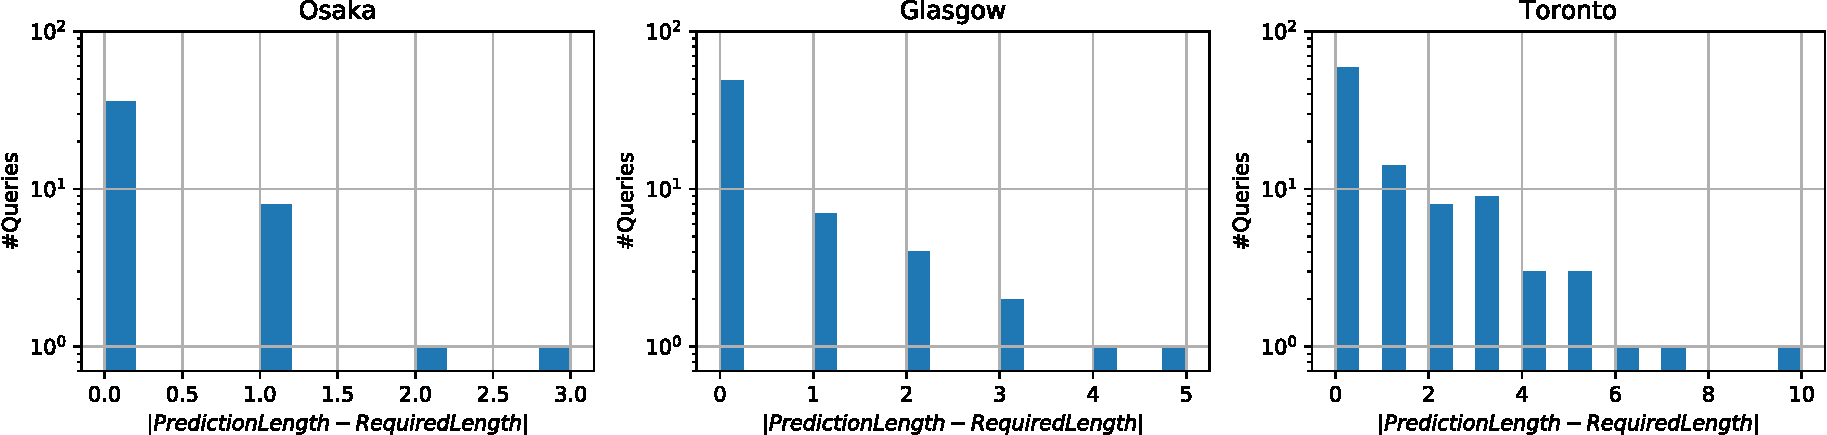
\includegraphics[width=0.95\textwidth]{heu_lengthdiff.pdf}
	    \captionof{figure}{Absolute difference between recommended and required sequence length for {\sc LoopElim(++)}.}
	    \label{fig:length-christo}
	    %\captionmoveup\eqmoveup
\end{figure*}%
\begin{figure*}[!t]
		\quad
		\centering
		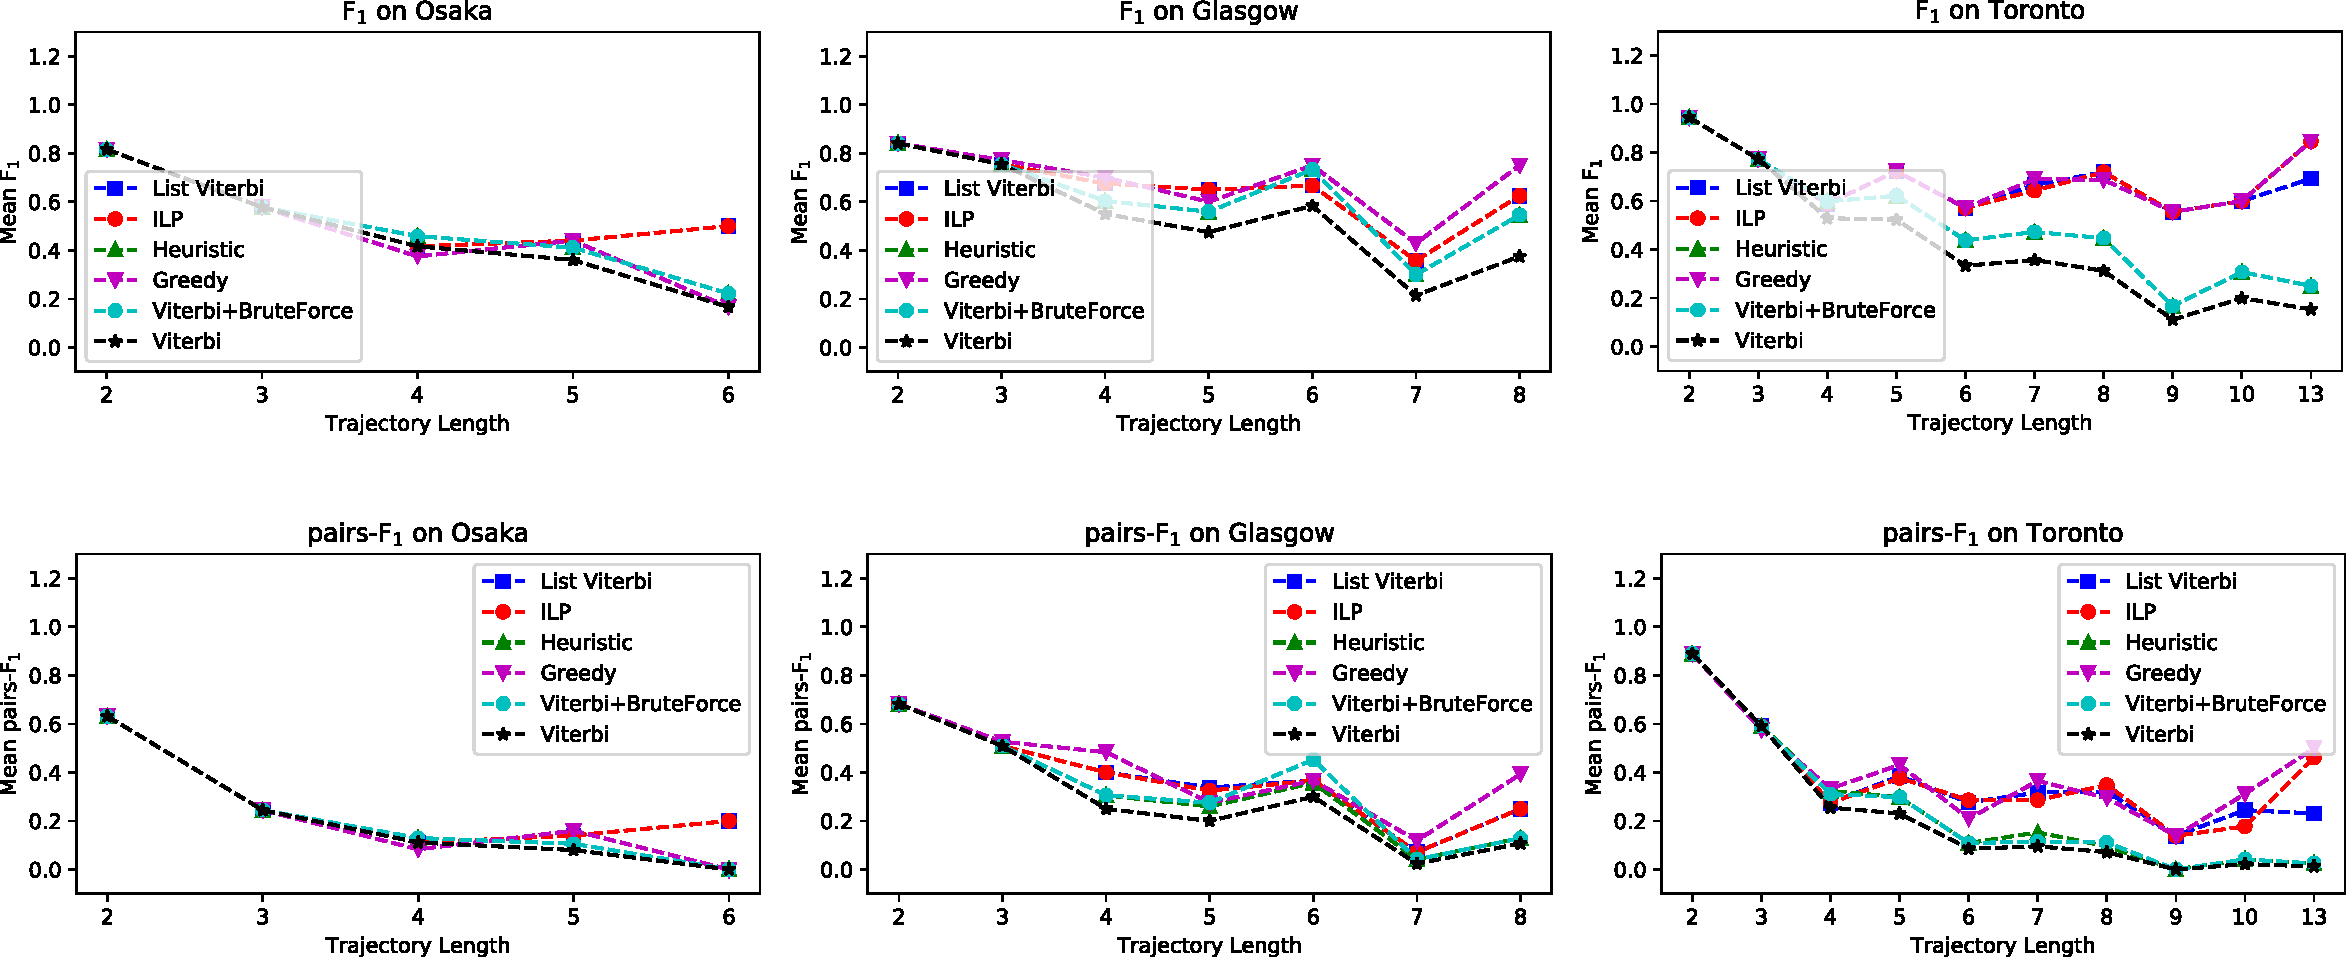
\includegraphics[width=0.95\textwidth]{metrics.pdf}
		% 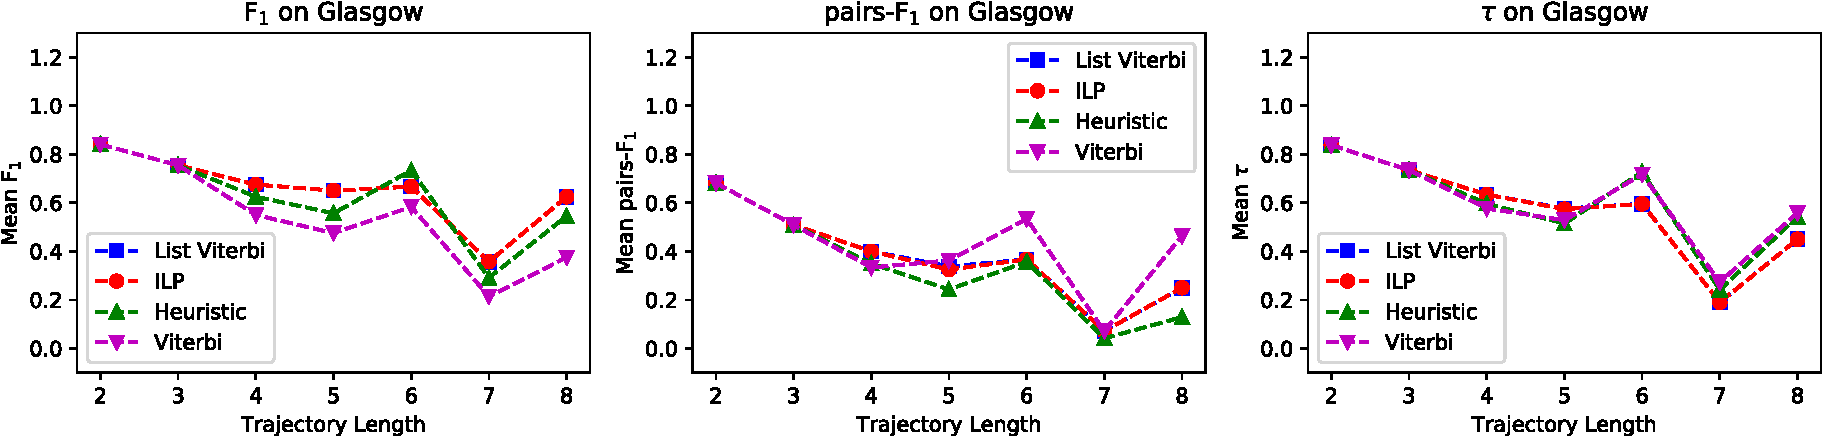
\includegraphics[width=\textwidth]{metric_d2.pdf}
		% 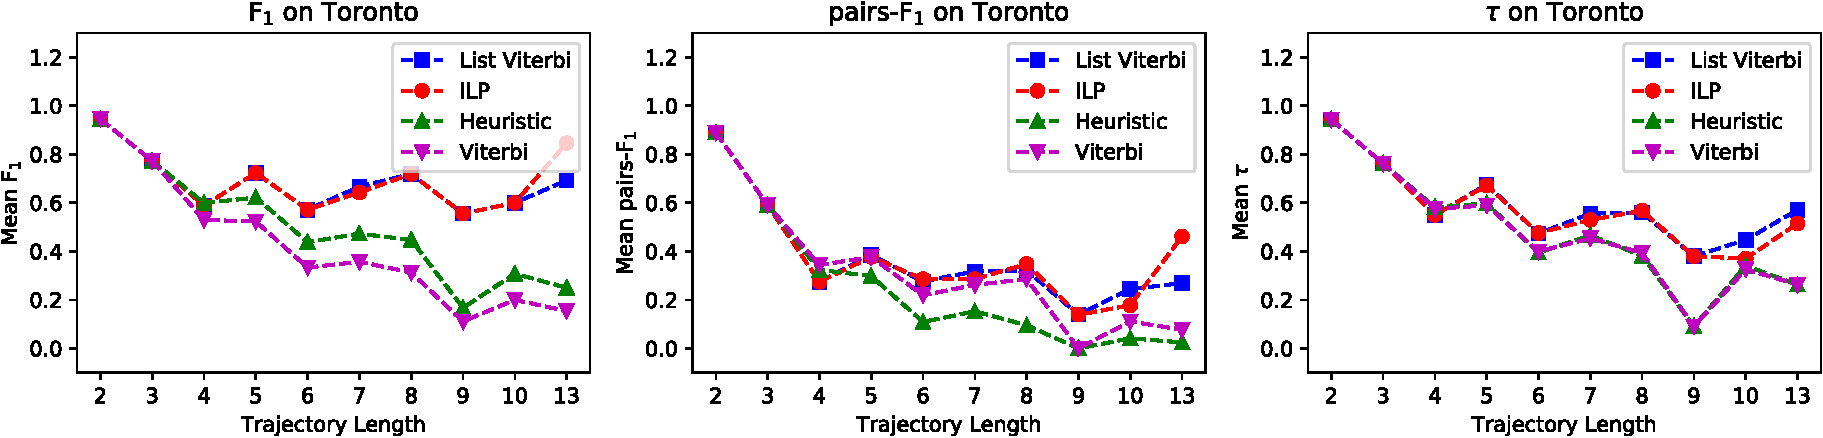
\includegraphics[width=\textwidth]{metric_d3.pdf}
	    \captionof{figure}{Accuracy versus trajectory length for all inference algorithms.}
	    \label{fig:acc-vs-length}
	    %\captionmoveup\eqmoveup
\end{figure*}%
\begin{figure*}[!t]
		\centering
		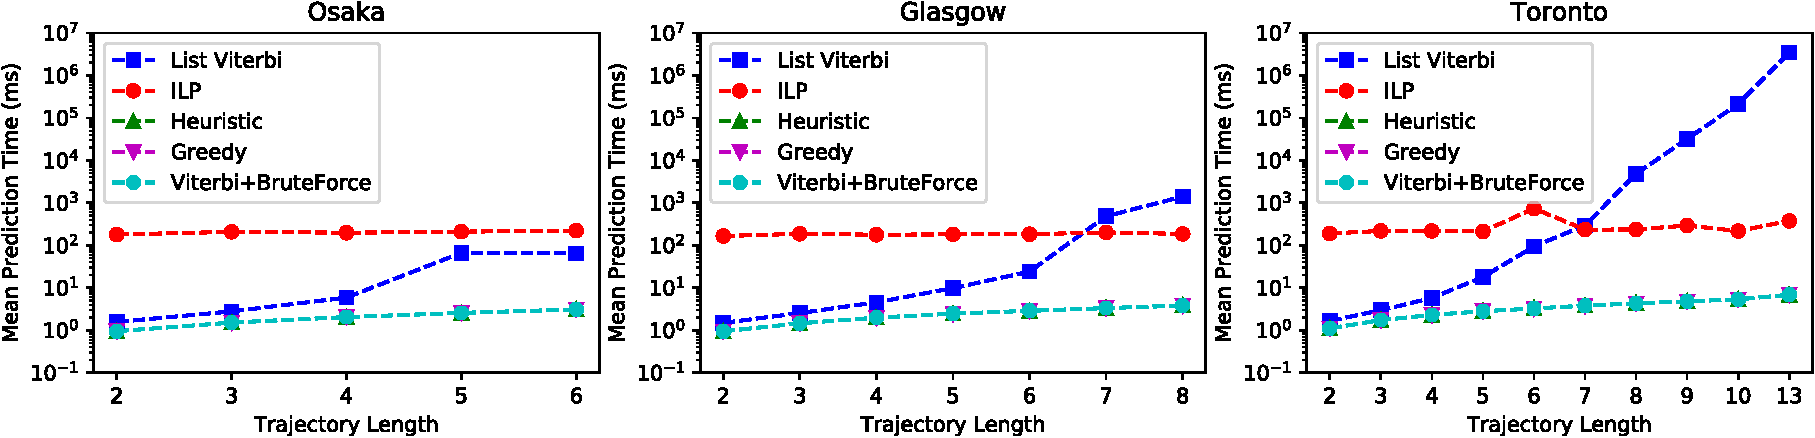
\includegraphics[width=0.95\textwidth]{top1_inftime.pdf}
	    \captionof{figure}{Prediction time versus trajectory length for all inference algorithms.}
	    \label{fig:inftime}
	    %\captionmoveup\eqmoveup
\end{figure*}%
% \end{minipage}
% \end{figure*}
